\section{Kernel Regression}

\begin{enumerate}
    \item Build the model. (auto-graded only)
    
    \item Analysis of the model.

Figures:
\begin{figure}[H]
  \caption{$\sigma = 0.01$}
  \centering
    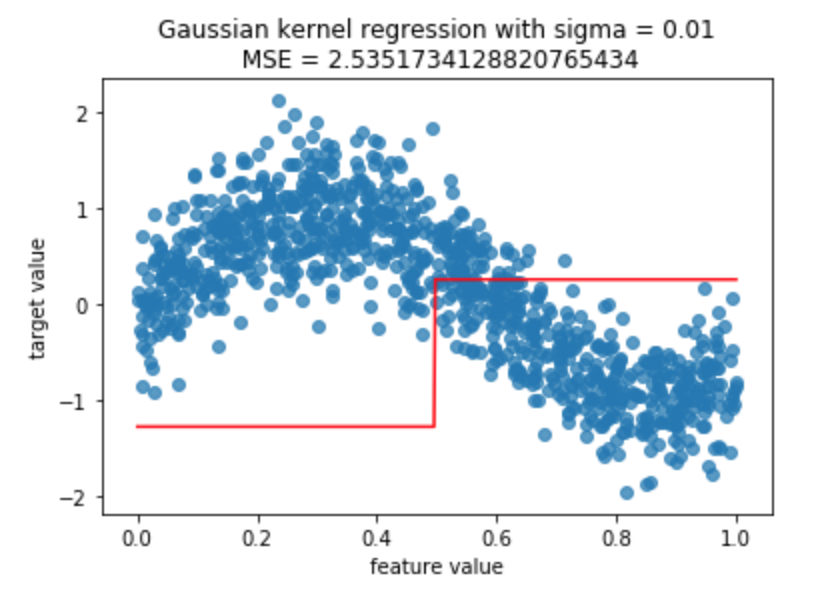
\includegraphics[width=0.5\textwidth]{images/1.png}
\end{figure}

\begin{figure}[H]
  \caption{$\sigma = 0.05$}
  \centering
    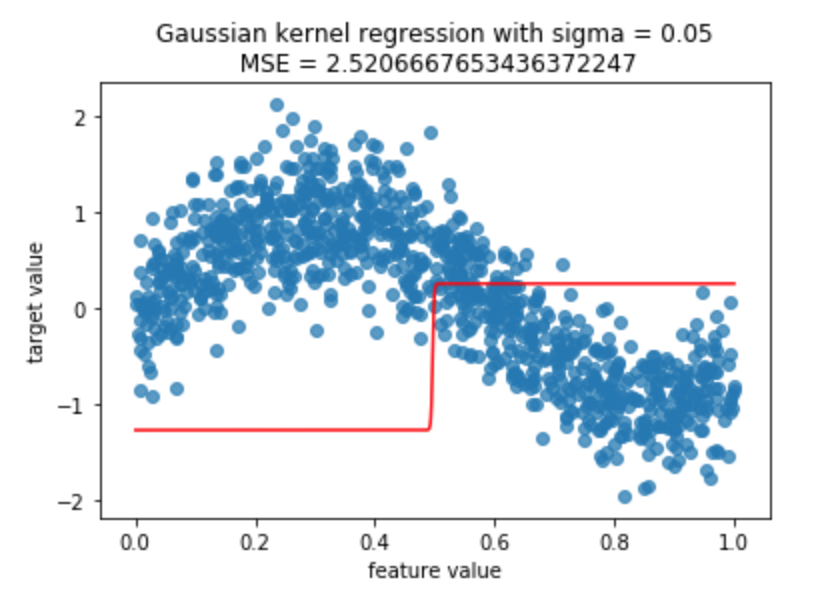
\includegraphics[width=0.5\textwidth]{images/2.png}
\end{figure}

\begin{figure}[H]
  \caption{$\sigma = 0.1$}
  \centering
    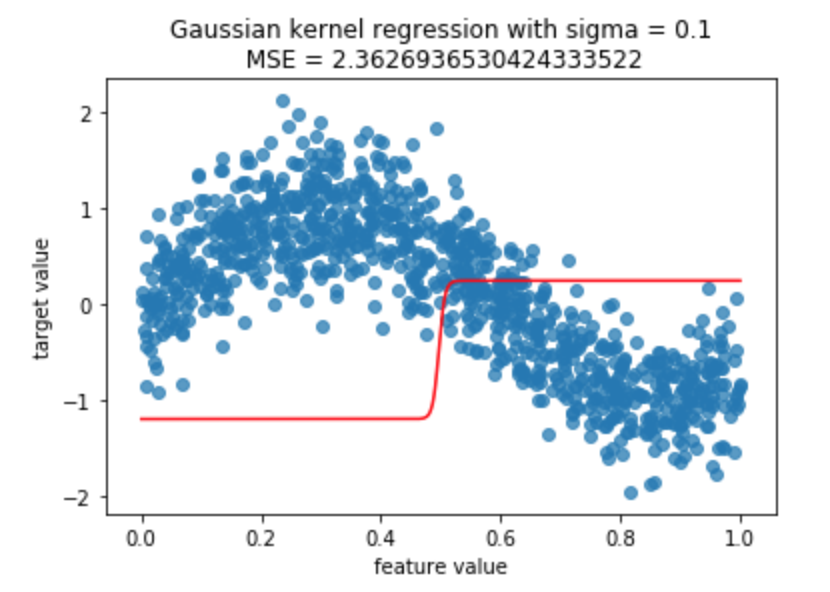
\includegraphics[width=0.5\textwidth]{images/3.png}
\end{figure}
    
\begin{figure}[H]
  \caption{$\sigma = 0.15$}
  \centering
    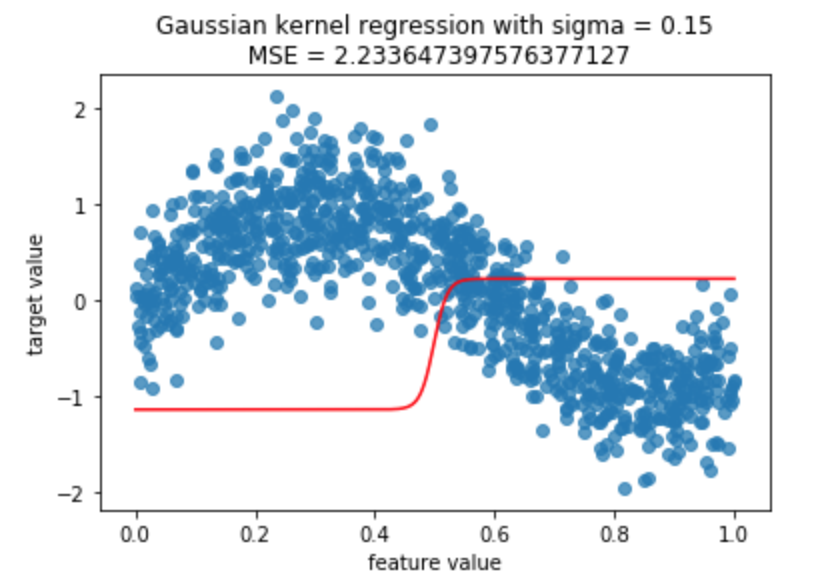
\includegraphics[width=0.5\textwidth]{images/4.png}
\end{figure}

\begin{figure}[H]
  \caption{$\sigma = 0.2$}
  \centering
    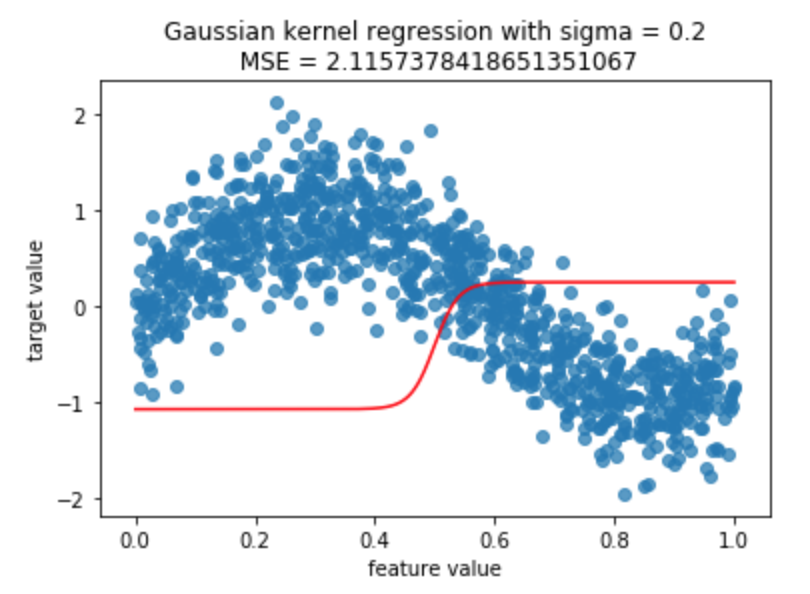
\includegraphics[width=0.5\textwidth]{images/5.png}
\end{figure}

\begin{figure}[H]
  \caption{$\sigma = 0.5$}
  \centering
    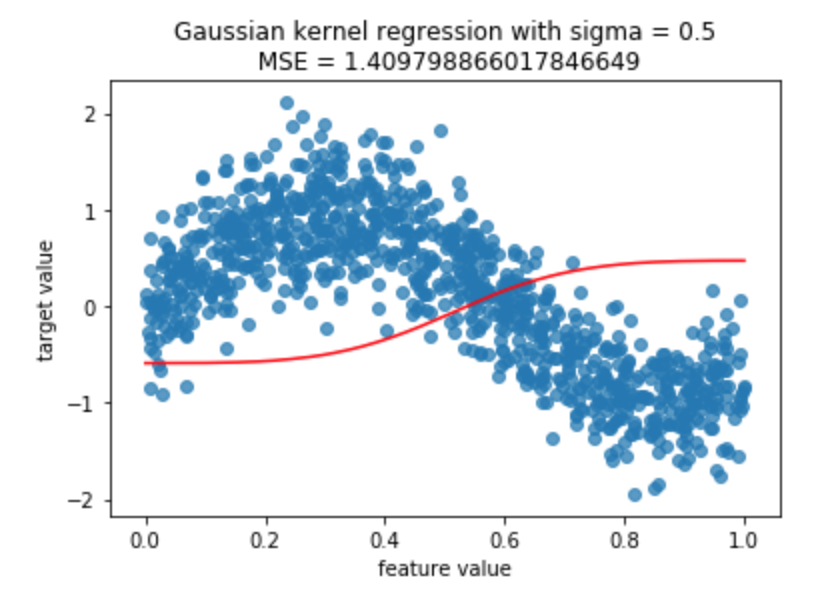
\includegraphics[width=0.5\textwidth]{images/6.png}
\end{figure}

\begin{figure}[H]
  \caption{$\sigma = 1.0$}
  \centering
    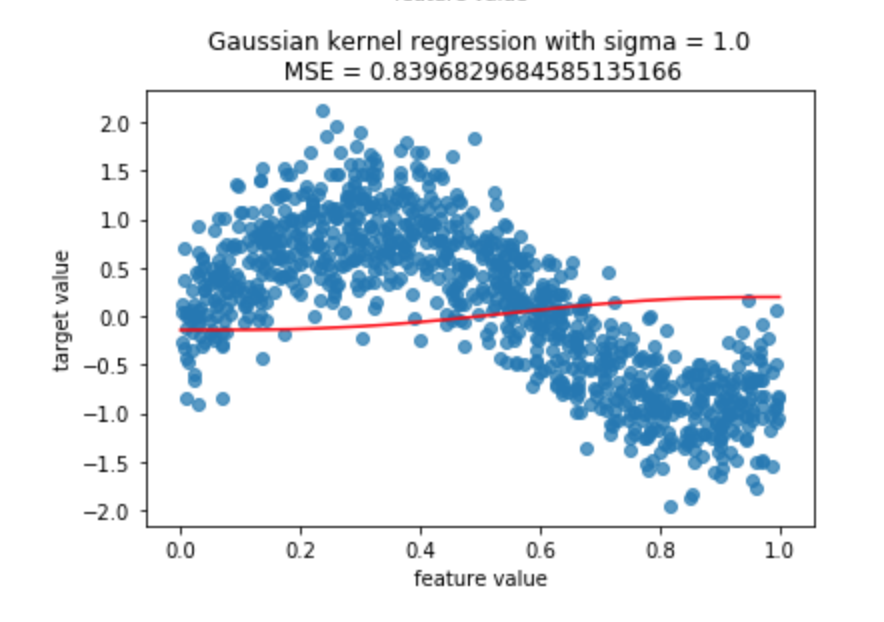
\includegraphics[width=0.5\textwidth]{images/7.png}
\end{figure}
Smallest MSE: 0.83968

Smallest MSE Sigma Value: 1.0

As sigma value is increasing the MSE is decreasing. As from the plots it is observed that training and predicted values are non-linear in nature, the trend is well captured as the sigma increases as it adds more non-linearity.

Learning curve of the model is improving with the increase of sigma value and error is decreasing.

\end{enumerate}